\section{Our process}\label{sprint1:ourprocess}
As described in \autoref{sec:essence}, a bi-focus of this project will be to attempt using the Essence process model as taught by the Software Innovation course.
We have been working with a ScrumBut approach in both previous semesters and at the beginning of this semester, but we decided that we wanted to try a new organization this semester, and as we learned more about the Essence approach we decided to pivot, changing our process. \\
However, we have chosen to keep sprints, stand-up meetings and retrospective meetings from Scrum as these can complement Essence.
To make the report fit this format, it has been split into the 4 sprints that we will go through during the semester, where each sprint has a length of 3 weeks.

\subsection{Roles}
We have divided the roles that were described in \autoref{sec:team-organization} between the members of the group.
One person has the \textit{Challenger} role, meaning that they are accountable for prioritizing the tasks in the backlog.
The process of prioritizing tasks is further described in the following section.
Another person has the \textit{Anchor} role, and is responsible for changes to the process and is in charge of leading evaluations of the process.
The rest of the group functions as \textit{Responders}, and are the developers of the project.
The \textit{Child} role fluctuates between members of the group.
Everyone can add suggestions to improve an idea and give other perspectives on the project. \\
Due to our team size, the challenger and anchor will also work as developers during the duration of the project.

\subsection{Prioritizing task}
Our backlog is saved as a board on Jira, which can be seen on \autoref{fig:to-do-board}.
The leftmost column is the \textit{Suggested} column.
Everyone can make suggestions for tasks that they find useful for the project.
After each stand-up meeting, the challenger will present new suggestions that seem relevant to work on in the near future.
This presentation will include the definition of done, and all members of the group will then vote on how valuable it is for the project and how time-consuming it is.
The priority of a task is then calculated as $reward - time$, which is an arbitrary number to indicate how important it is.
\\\\
The challenger then chooses the most important features from the \textit{Discussed} column, often based on the highest priority, as \textit{Chosen for Development}.
Responders then have the opportunity to take tasks from this column and move it to the next column \textit{In progress} when they start working on it.
When the task has been completed, reviewed and merged into the develop branch, it is automatically moved to the column \textit{Done}.
\begin{figure}[H]
    \centering
    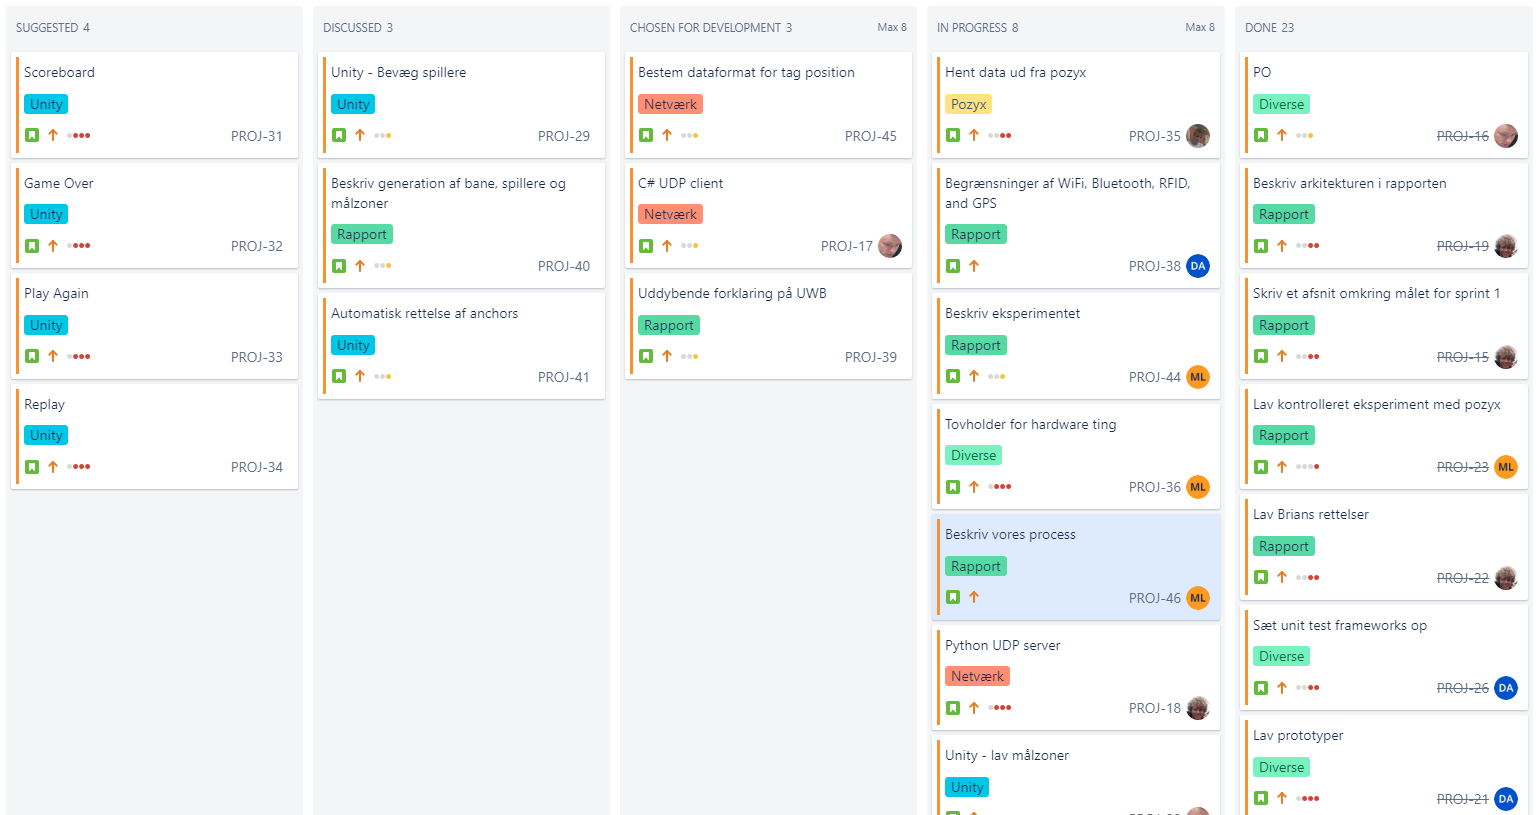
\includegraphics[width=\linewidth]{kanban.PNG}
    \caption{The board for tasks.}
    \label{fig:to-do-board}
\end{figure}

\subsection{Pair reviews}
To ensure quality and make sure that people follow the test plan, everything undergoes a formal review before it is added to the project.
For report tasks, they are assigned to review and accept it before it can be merged.
For coding tasks, two people are likewise assigned to review it, but the review has to be done as a pair, meaning that they have to physically sit together and go through the code on a shared screen.
These pair reviews are a good way to share knowledge about the implementation through the group, as people have to understand it to be able to discuss it.
In previous semesters people have reviewed the code separately, which leads to fewer comments as the code was not discussed between reviewers.
